\documentclass{standalone}
\usepackage{tikz}
\usetikzlibrary{patterns, positioning}
\usepackage[sfdefault]{ClearSans} %% option 'sfdefault' activates Clear Sans as the default text font
\usepackage[T1]{fontenc}

\begin{document}
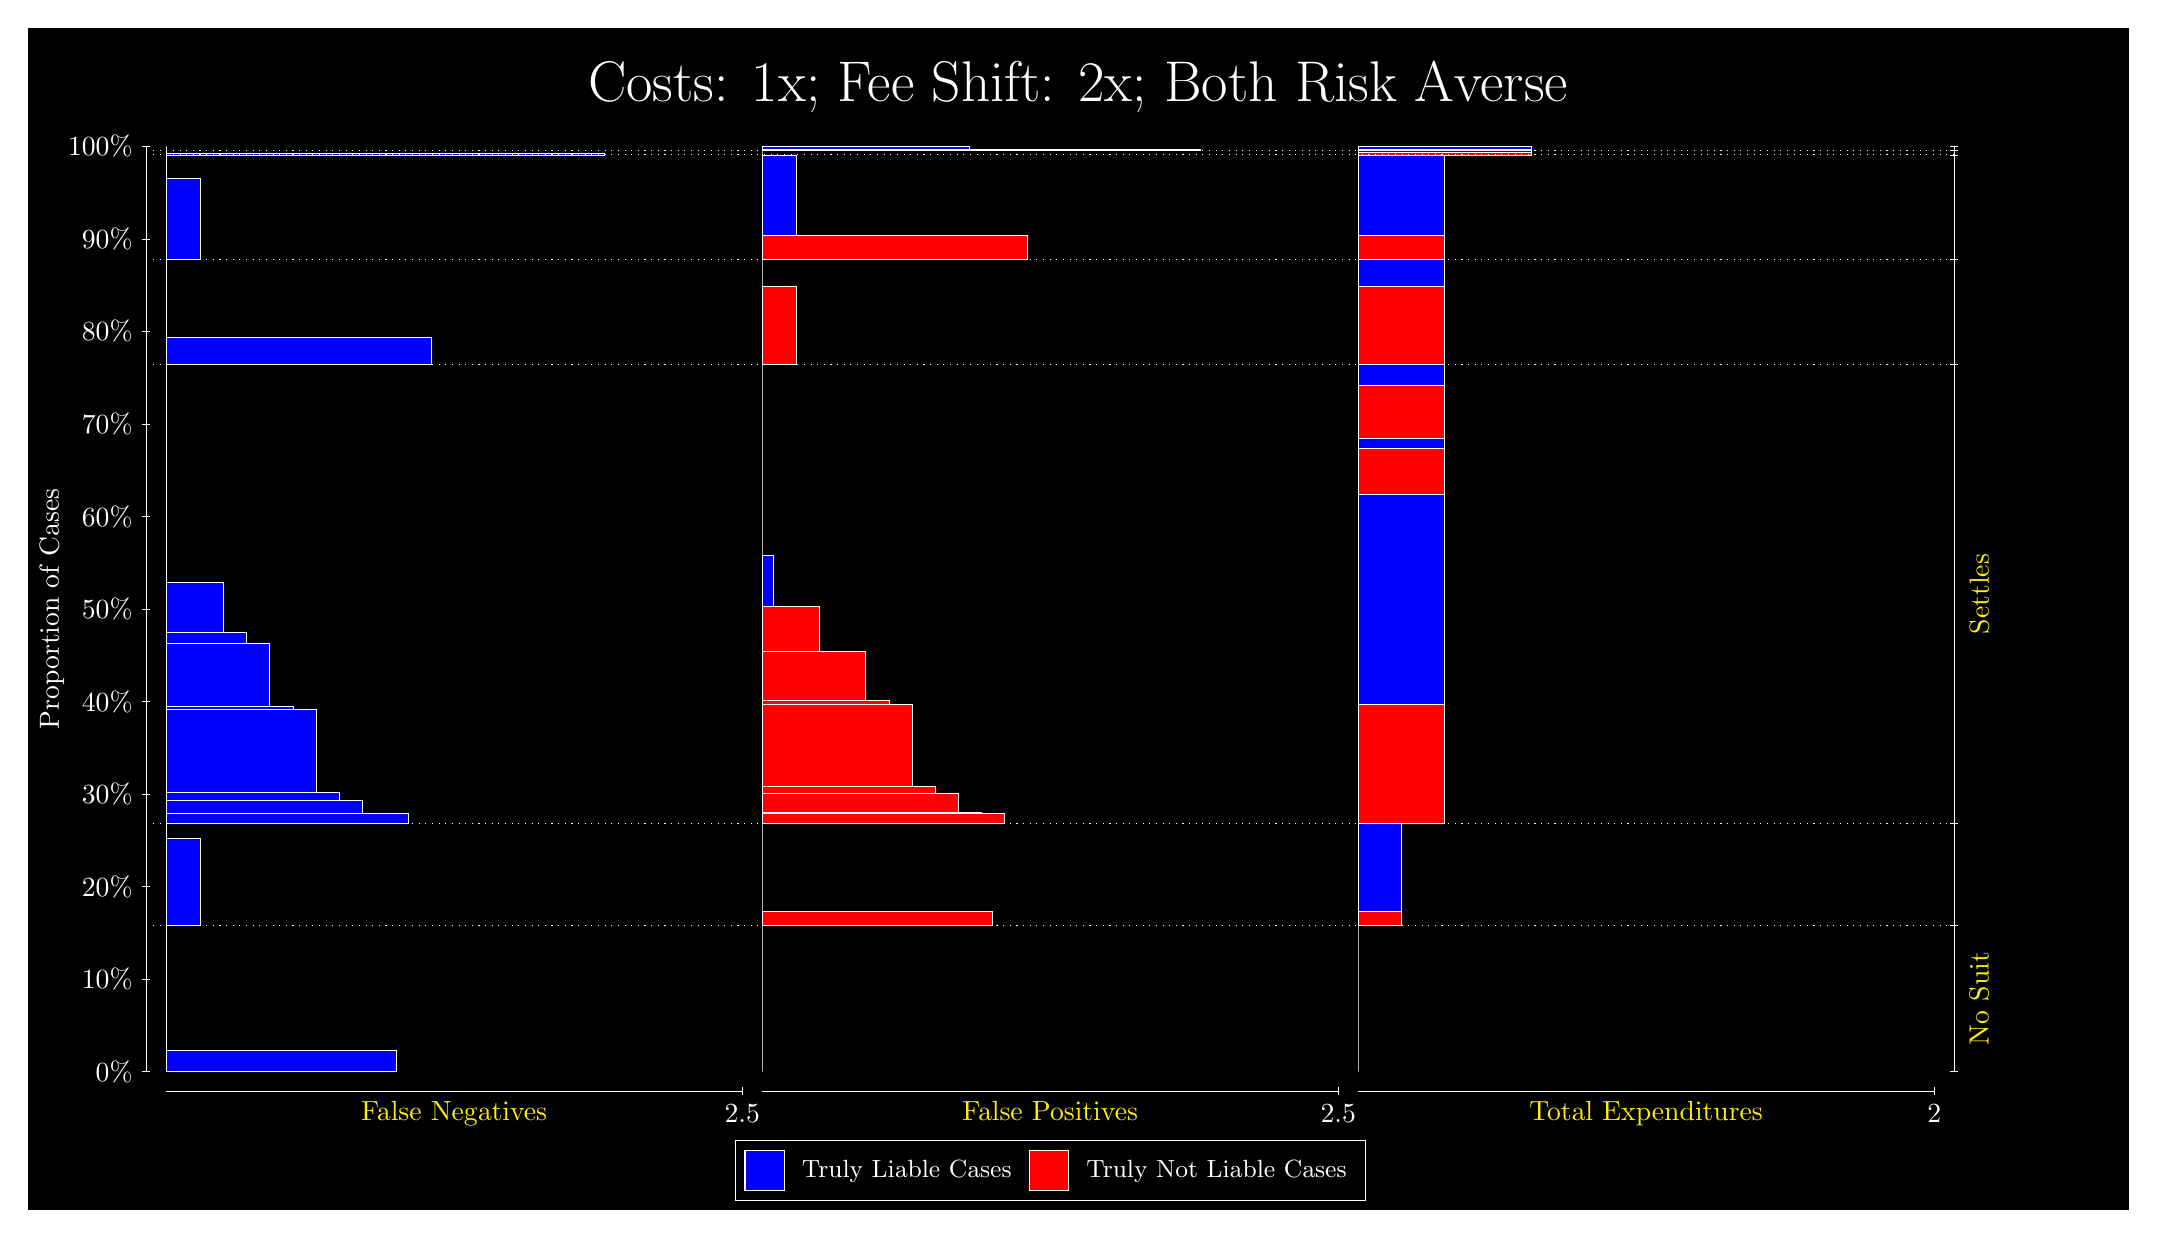
\begin{tikzpicture}
\draw[fill=black] (0,0) rectangle (26.667,15);
\draw[text=white] (0,13.5) rectangle (26.667,15) node[midway] {\huge Costs: 1x; Fee Shift: 2x; Both Risk Averse};
\draw[white, very thin] (1.5,1.75) -- (1.5,13.5);
\node[rotate=90, text=white, anchor=center] at (0.3, 7.625) {Proportion of Cases};
\draw[white, very thin] (1.45,1.75) -- (1.55,1.75);
\node[text=white, anchor=east] at (1.45, 1.75) {0\%};
\draw[white, very thin] (1.45,2.925) -- (1.55,2.925);
\node[text=white, anchor=east] at (1.45, 2.925) {10\%};
\draw[white, very thin] (1.45,4.1) -- (1.55,4.1);
\node[text=white, anchor=east] at (1.45, 4.1) {20\%};
\draw[white, very thin] (1.45,5.275) -- (1.55,5.275);
\node[text=white, anchor=east] at (1.45, 5.275) {30\%};
\draw[white, very thin] (1.45,6.45) -- (1.55,6.45);
\node[text=white, anchor=east] at (1.45, 6.45) {40\%};
\draw[white, very thin] (1.45,7.625) -- (1.55,7.625);
\node[text=white, anchor=east] at (1.45, 7.625) {50\%};
\draw[white, very thin] (1.45,8.8) -- (1.55,8.8);
\node[text=white, anchor=east] at (1.45, 8.8) {60\%};
\draw[white, very thin] (1.45,9.975) -- (1.55,9.975);
\node[text=white, anchor=east] at (1.45, 9.975) {70\%};
\draw[white, very thin] (1.45,11.15) -- (1.55,11.15);
\node[text=white, anchor=east] at (1.45, 11.15) {80\%};
\draw[white, very thin] (1.45,12.325) -- (1.55,12.325);
\node[text=white, anchor=east] at (1.45, 12.325) {90\%};
\draw[white, very thin] (1.45,13.5) -- (1.55,13.5);
\node[text=white, anchor=east] at (1.45, 13.5) {100\%};

\draw[white, very thin] (24.457,1.75) -- (24.457,13.5);
\draw[white, very thin] (24.407,1.75) -- (24.507,1.75);
\node[anchor=west] at (24.407, 1.75) {};
\draw[white, very thin] (24.407,3.6052) -- (24.507,3.6052);
\node[anchor=west] at (24.407, 3.6052) {};
\draw[white, very thin] (24.407,4.8986) -- (24.507,4.8986);
\node[anchor=west] at (24.407, 4.8986) {};
\draw[white, very thin] (24.407,10.728) -- (24.507,10.728);
\node[anchor=west] at (24.407, 10.728) {};
\draw[white, very thin] (24.407,12.068) -- (24.507,12.068);
\node[anchor=west] at (24.407, 12.068) {};
\draw[white, very thin] (24.407,13.392) -- (24.507,13.392);
\node[anchor=west] at (24.407, 13.392) {};
\draw[white, very thin] (24.407,13.444) -- (24.507,13.444);
\node[anchor=west] at (24.407, 13.444) {};
\draw[white, very thin] (24.407,13.5) -- (24.507,13.5);
\node[anchor=west] at (24.407, 13.5) {};

\draw[white, very thin, fill=blue] (1.75,1.75) rectangle (4.6775,2.0212);
\draw[white, very thin, fill=red] (1.75,2.0212) rectangle (1.75,3.6052);
\draw[white, very thin, fill=blue] (1.75,3.6052) rectangle (2.1891,4.7178);
\draw[white, very thin, fill=red] (1.75,4.7178) rectangle (1.75,4.8986);
\draw[white, very thin, fill=blue] (1.75,4.8986) rectangle (4.8239,5.0336);
\draw[white, very thin, fill=blue] (1.75,5.0336) rectangle (4.2384,5.2004);
\draw[white, very thin, fill=blue] (1.75,5.2004) rectangle (3.9457,5.2981);
\draw[white, very thin, fill=blue] (1.75,5.2981) rectangle (3.6529,6.3486);
\draw[white, very thin, fill=blue] (1.75,6.3486) rectangle (3.3602,6.3866);
\draw[white, very thin, fill=blue] (1.75,6.3866) rectangle (3.0674,7.1863);
\draw[white, very thin, fill=blue] (1.75,7.1863) rectangle (2.7746,7.3261);
\draw[white, very thin, fill=blue] (1.75,7.3261) rectangle (2.4819,7.9633);
\draw[white, very thin, fill=red] (1.75,7.9633) rectangle (1.75,10.728);
\draw[white, very thin, fill=blue] (1.75,10.728) rectangle (5.1167,11.073);
\draw[white, very thin, fill=red] (1.75,11.073) rectangle (1.75,12.068);
\draw[white, very thin, fill=blue] (1.75,12.068) rectangle (2.1891,13.093);
\draw[white, very thin, fill=red] (1.75,13.093) rectangle (1.75,13.392);
\draw[white, very thin, fill=blue] (1.75,13.392) rectangle (7.3123,13.409);
\draw[white, very thin, fill=red] (1.75,13.409) rectangle (1.75,13.444);
\draw[white, very thin, fill=red] (1.75,13.444) rectangle (1.75,13.461);
\draw[white, very thin, fill=blue] (1.75,13.461) rectangle (1.75,13.5);
\draw[white, very thin, fill=red] (9.3189,1.75) rectangle (9.3189,3.3339);
\draw[white, very thin, fill=blue] (9.3189,3.3339) rectangle (9.3189,3.6052);
\draw[white, very thin, fill=red] (9.3189,3.6052) rectangle (12.246,3.786);
\draw[white, very thin, fill=blue] (9.3189,3.786) rectangle (9.3189,4.8986);
\draw[white, very thin, fill=red] (9.3189,4.8986) rectangle (12.393,5.028);
\draw[white, very thin, fill=red] (9.3189,5.028) rectangle (12.1,5.047);
\draw[white, very thin, fill=red] (9.3189,5.047) rectangle (11.807,5.2802);
\draw[white, very thin, fill=red] (9.3189,5.2802) rectangle (11.515,5.3702);
\draw[white, very thin, fill=red] (9.3189,5.3702) rectangle (11.222,6.4193);
\draw[white, very thin, fill=red] (9.3189,6.4193) rectangle (10.929,6.4676);
\draw[white, very thin, fill=red] (9.3189,6.4676) rectangle (10.636,7.0854);
\draw[white, very thin, fill=red] (9.3189,7.0854) rectangle (10.051,7.6634);
\draw[white, very thin, fill=blue] (9.3189,7.6634) rectangle (9.4652,8.3007);
\draw[white, very thin, fill=blue] (9.3189,8.3007) rectangle (9.3189,10.728);
\draw[white, very thin, fill=red] (9.3189,10.728) rectangle (9.758,11.723);
\draw[white, very thin, fill=blue] (9.3189,11.723) rectangle (9.3189,12.068);
\draw[white, very thin, fill=red] (9.3189,12.068) rectangle (12.686,12.367);
\draw[white, very thin, fill=blue] (9.3189,12.367) rectangle (9.758,13.392);
\draw[white, very thin, fill=red] (9.3189,13.392) rectangle (9.3189,13.427);
\draw[white, very thin, fill=blue] (9.3189,13.427) rectangle (9.3189,13.444);
\draw[white, very thin, fill=red] (9.3189,13.444) rectangle (14.881,13.461);
\draw[white, very thin, fill=blue] (9.3189,13.461) rectangle (11.954,13.5);
\draw[white, very thin, fill=red] (16.888,1.75) rectangle (16.888,3.3339);
\draw[white, very thin, fill=blue] (16.888,3.3339) rectangle (16.888,3.6052);
\draw[white, very thin, fill=red] (16.888,3.6052) rectangle (17.437,3.786);
\draw[white, very thin, fill=blue] (16.888,3.786) rectangle (17.437,4.8986);
\draw[white, very thin, fill=red] (16.888,4.8986) rectangle (17.986,6.4193);
\draw[white, very thin, fill=blue] (16.888,6.4193) rectangle (17.986,9.0845);
\draw[white, very thin, fill=red] (16.888,9.0845) rectangle (17.986,9.6626);
\draw[white, very thin, fill=blue] (16.888,9.6626) rectangle (17.986,9.7976);
\draw[white, very thin, fill=red] (16.888,9.7976) rectangle (17.986,10.464);
\draw[white, very thin, fill=blue] (16.888,10.464) rectangle (17.986,10.728);
\draw[white, very thin, fill=red] (16.888,10.728) rectangle (17.986,11.723);
\draw[white, very thin, fill=blue] (16.888,11.723) rectangle (17.986,12.068);
\draw[white, very thin, fill=red] (16.888,12.068) rectangle (17.986,12.367);
\draw[white, very thin, fill=blue] (16.888,12.367) rectangle (17.986,13.392);
\draw[white, very thin, fill=red] (16.888,13.392) rectangle (19.083,13.427);
\draw[white, very thin, fill=blue] (16.888,13.427) rectangle (19.083,13.444);
\draw[white, very thin, fill=red] (16.888,13.444) rectangle (19.083,13.461);
\draw[white, very thin, fill=blue] (16.888,13.461) rectangle (19.083,13.5);
\draw[white, dotted] (1.5,3.6052) -- (24.457,3.6052);
\draw[white, dotted] (1.5,4.8986) -- (24.457,4.8986);
\draw[white, dotted] (1.5,10.728) -- (24.457,10.728);
\draw[white, dotted] (1.5,12.068) -- (24.457,12.068);
\draw[white, dotted] (1.5,13.392) -- (24.457,13.392);
\draw[white, dotted] (1.5,13.444) -- (24.457,13.444);
\draw[white, very thin] (1.75,1.5) -- (9.0689,1.5);
\node[text=yellow, anchor=north] at (5.4094, 1.5) {False Negatives};
\draw[white, very thin] (9.0689,1.45) -- (9.0689,1.55);
\node[text=white, anchor=north] at (9.0689, 1.45) {2.5};

\draw[white, very thin] (9.3189,1.5) -- (16.638,1.5);
\node[text=yellow, anchor=north] at (12.978, 1.5) {False Positives};
\draw[white, very thin] (16.638,1.45) -- (16.638,1.55);
\node[text=white, anchor=north] at (16.638, 1.45) {2.5};

\draw[white, very thin] (16.888,1.5) -- (24.207,1.5);
\node[text=yellow, anchor=north] at (20.547, 1.5) {Total Expenditures};
\draw[white, very thin] (24.207,1.45) -- (24.207,1.55);
\node[text=white, anchor=north] at (24.207, 1.45) {2};

\node[text=yellow, centered, rotate=90] at (24.777, 2.6776) {No Suit};

\node[text=yellow, centered, rotate=90] at (24.777, 7.8134) {Settles};





\draw (12.978300999999998,1.5) node[draw=none] (baseCoordinate) {};
\begin{scope}[align=center]
        \matrix[scale=0.5, draw=white, below=0.5cm of baseCoordinate, nodes={draw}, column sep=0.1cm]{
            \node[rectangle, draw, minimum width=0.5cm, minimum height=0.5cm, fill=blue] {}; &
            \node[draw=none, font=\small, text=white] (B) {Truly Liable Cases}; &
            \node[rectangle, draw, minimum width=0.5cm, minimum height=0.5cm, fill=red] {}; &
            \node[draw=none, font=\small, text=white] (B) {Truly Not Liable Cases}; \\
            };
\end{scope}

\end{tikzpicture}
\end{document}